% Created by tikzDevice version 0.12.6 on 2026-01-28 16:24:46
% !TEX encoding = UTF-8 Unicode
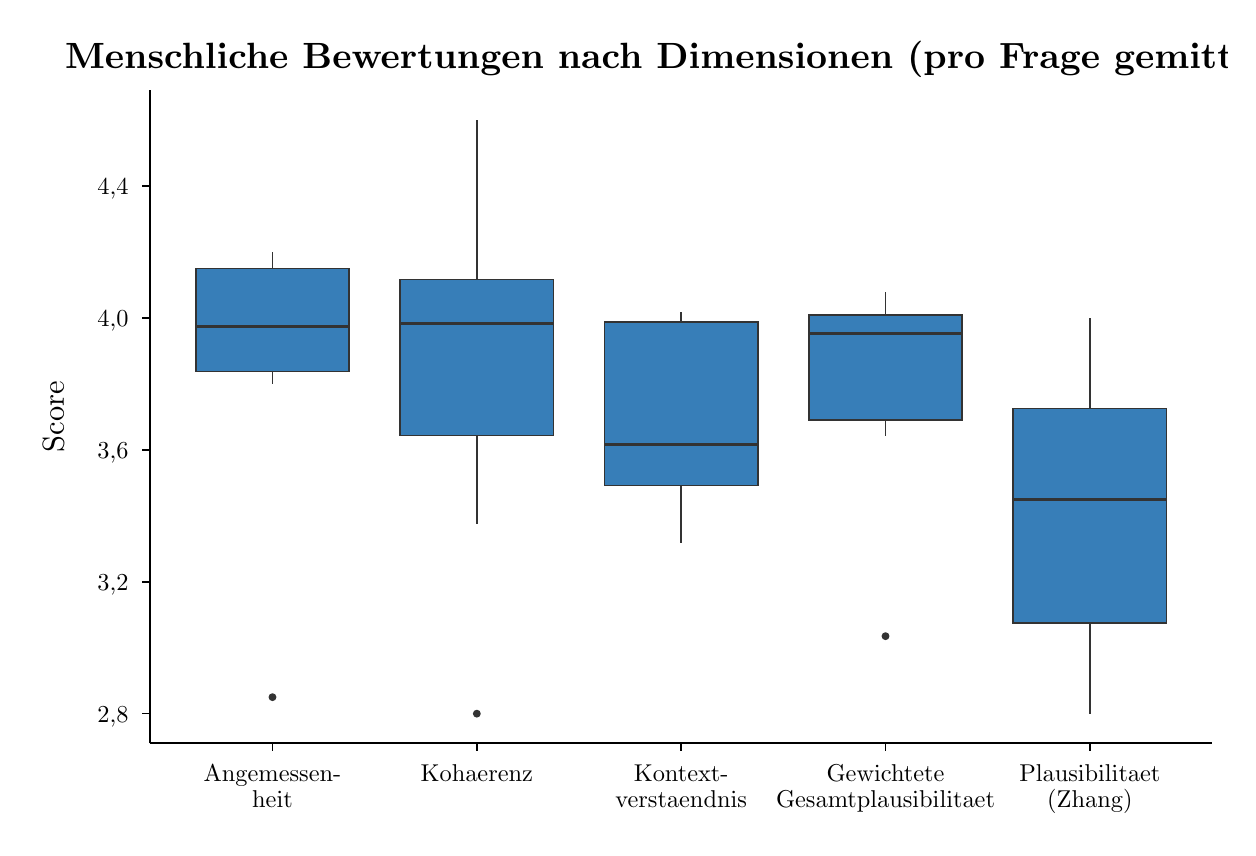
\begin{tikzpicture}[x=1pt,y=1pt]
\definecolor{fillColor}{RGB}{255,255,255}
\path[use as bounding box,fill=fillColor,fill opacity=0.00] (0,0) rectangle (433.62,289.08);
\begin{scope}
\path[clip] (  0.00,  0.00) rectangle (433.62,289.08);
\definecolor{fillColor}{RGB}{255,255,255}

\path[fill=fillColor] (  0.00,  0.00) rectangle (433.62,289.08);
\end{scope}
\begin{scope}
\path[clip] ( 44.16, 30.48) rectangle (428.12,266.40);
\definecolor{drawColor}{gray}{0.20}
\definecolor{fillColor}{gray}{0.20}

\path[draw=drawColor,line width= 0.4pt,line join=round,line cap=round,fill=fillColor] ( 88.46, 47.16) circle (  1.21);

\path[draw=drawColor,line width= 0.6pt,line join=round] ( 88.46,202.06) -- ( 88.46,208.02);

\path[draw=drawColor,line width= 0.6pt,line join=round] ( 88.46,164.82) -- ( 88.46,160.36);
\definecolor{fillColor}{RGB}{55,126,184}

\path[draw=drawColor,line width= 0.6pt,fill=fillColor] ( 60.77,202.06) --
	( 60.77,164.82) --
	(116.15,164.82) --
	(116.15,202.06) --
	( 60.77,202.06) --
	cycle;

\path[draw=drawColor,line width= 1.1pt] ( 60.77,181.21) -- (116.15,181.21);
\definecolor{fillColor}{gray}{0.20}

\path[draw=drawColor,line width= 0.4pt,line join=round,line cap=round,fill=fillColor] (162.30, 41.20) circle (  1.21);

\path[draw=drawColor,line width= 0.6pt,line join=round] (162.30,198.09) -- (162.30,255.68);

\path[draw=drawColor,line width= 0.6pt,line join=round] (162.30,141.74) -- (162.30,109.71);
\definecolor{fillColor}{RGB}{55,126,184}

\path[draw=drawColor,line width= 0.6pt,fill=fillColor] (134.61,198.09) --
	(134.61,141.74) --
	(189.99,141.74) --
	(189.99,198.09) --
	(134.61,198.09) --
	cycle;

\path[draw=drawColor,line width= 1.1pt] (134.61,182.20) -- (189.99,182.20);

\path[draw=drawColor,line width= 0.6pt,line join=round] (236.14,182.70) -- (236.14,186.17);

\path[draw=drawColor,line width= 0.6pt,line join=round] (236.14,123.62) -- (236.14,102.76);

\path[draw=drawColor,line width= 0.6pt,fill=fillColor] (208.45,182.70) --
	(208.45,123.62) --
	(263.83,123.62) --
	(263.83,182.70) --
	(208.45,182.70) --
	cycle;

\path[draw=drawColor,line width= 1.1pt] (208.45,138.51) -- (263.83,138.51);
\definecolor{fillColor}{gray}{0.20}

\path[draw=drawColor,line width= 0.4pt,line join=round,line cap=round,fill=fillColor] (309.98, 69.20) circle (  1.21);

\path[draw=drawColor,line width= 0.6pt,line join=round] (309.98,185.28) -- (309.98,193.72);

\path[draw=drawColor,line width= 0.6pt,line join=round] (309.98,147.20) -- (309.98,141.69);
\definecolor{fillColor}{RGB}{55,126,184}

\path[draw=drawColor,line width= 0.6pt,fill=fillColor] (282.29,185.28) --
	(282.29,147.20) --
	(337.67,147.20) --
	(337.67,185.28) --
	(282.29,185.28) --
	cycle;

\path[draw=drawColor,line width= 1.1pt] (282.29,178.63) -- (337.67,178.63);

\path[draw=drawColor,line width= 0.6pt,line join=round] (383.82,151.42) -- (383.82,184.19);

\path[draw=drawColor,line width= 0.6pt,line join=round] (383.82, 73.97) -- (383.82, 41.20);

\path[draw=drawColor,line width= 0.6pt,fill=fillColor] (356.13,151.42) --
	(356.13, 73.97) --
	(411.51, 73.97) --
	(411.51,151.42) --
	(356.13,151.42) --
	cycle;

\path[draw=drawColor,line width= 1.1pt] (356.13,118.65) -- (411.51,118.65);
\end{scope}
\begin{scope}
\path[clip] (  0.00,  0.00) rectangle (433.62,289.08);
\definecolor{drawColor}{RGB}{0,0,0}

\path[draw=drawColor,line width= 0.6pt,line join=round] ( 44.16, 30.48) --
	( 44.16,266.40);
\end{scope}
\begin{scope}
\path[clip] (  0.00,  0.00) rectangle (433.62,289.08);
\definecolor{drawColor}{RGB}{0,0,0}

\node[text=drawColor,anchor=base east,inner sep=0pt, outer sep=0pt, scale=  0.88] at ( 36.46, 38.17) {2,8};

\node[text=drawColor,anchor=base east,inner sep=0pt, outer sep=0pt, scale=  0.88] at ( 36.46, 85.83) {3,2};

\node[text=drawColor,anchor=base east,inner sep=0pt, outer sep=0pt, scale=  0.88] at ( 36.46,133.49) {3,6};

\node[text=drawColor,anchor=base east,inner sep=0pt, outer sep=0pt, scale=  0.88] at ( 36.46,181.16) {4,0};

\node[text=drawColor,anchor=base east,inner sep=0pt, outer sep=0pt, scale=  0.88] at ( 36.46,228.82) {4,4};
\end{scope}
\begin{scope}
\path[clip] (  0.00,  0.00) rectangle (433.62,289.08);
\definecolor{drawColor}{RGB}{0,0,0}

\path[draw=drawColor,line width= 0.6pt,line join=round] ( 41.41, 41.20) --
	( 44.16, 41.20);

\path[draw=drawColor,line width= 0.6pt,line join=round] ( 41.41, 88.86) --
	( 44.16, 88.86);

\path[draw=drawColor,line width= 0.6pt,line join=round] ( 41.41,136.52) --
	( 44.16,136.52);

\path[draw=drawColor,line width= 0.6pt,line join=round] ( 41.41,184.19) --
	( 44.16,184.19);

\path[draw=drawColor,line width= 0.6pt,line join=round] ( 41.41,231.85) --
	( 44.16,231.85);
\end{scope}
\begin{scope}
\path[clip] (  0.00,  0.00) rectangle (433.62,289.08);
\definecolor{drawColor}{RGB}{0,0,0}

\path[draw=drawColor,line width= 0.6pt,line join=round] ( 44.16, 30.48) --
	(428.12, 30.48);
\end{scope}
\begin{scope}
\path[clip] (  0.00,  0.00) rectangle (433.62,289.08);
\definecolor{drawColor}{RGB}{0,0,0}

\path[draw=drawColor,line width= 0.6pt,line join=round] ( 88.46, 27.73) --
	( 88.46, 30.48);

\path[draw=drawColor,line width= 0.6pt,line join=round] (162.30, 27.73) --
	(162.30, 30.48);

\path[draw=drawColor,line width= 0.6pt,line join=round] (236.14, 27.73) --
	(236.14, 30.48);

\path[draw=drawColor,line width= 0.6pt,line join=round] (309.98, 27.73) --
	(309.98, 30.48);

\path[draw=drawColor,line width= 0.6pt,line join=round] (383.82, 27.73) --
	(383.82, 30.48);
\end{scope}
\begin{scope}
\path[clip] (  0.00,  0.00) rectangle (433.62,289.08);
\definecolor{drawColor}{RGB}{0,0,0}

\node[text=drawColor,anchor=base,inner sep=0pt, outer sep=0pt, scale=  0.88] at ( 88.46, 16.71) {Angemessen-};

\node[text=drawColor,anchor=base,inner sep=0pt, outer sep=0pt, scale=  0.88] at ( 88.46,  7.21) {heit};

\node[text=drawColor,anchor=base,inner sep=0pt, outer sep=0pt, scale=  0.88] at (162.30, 16.71) {Kohaerenz};

\node[text=drawColor,anchor=base,inner sep=0pt, outer sep=0pt, scale=  0.88] at (236.14, 16.71) {Kontext-};

\node[text=drawColor,anchor=base,inner sep=0pt, outer sep=0pt, scale=  0.88] at (236.14,  7.21) {verstaendnis};

\node[text=drawColor,anchor=base,inner sep=0pt, outer sep=0pt, scale=  0.88] at (309.98, 16.71) {Gewichtete};

\node[text=drawColor,anchor=base,inner sep=0pt, outer sep=0pt, scale=  0.88] at (309.98,  7.21) {Gesamtplausibilitaet};

\node[text=drawColor,anchor=base,inner sep=0pt, outer sep=0pt, scale=  0.88] at (383.82, 16.71) {Plausibilitaet};

\node[text=drawColor,anchor=base,inner sep=0pt, outer sep=0pt, scale=  0.88] at (383.82,  7.21) {(Zhang)};
\end{scope}
\begin{scope}
\path[clip] (  0.00,  0.00) rectangle (433.62,289.08);
\definecolor{drawColor}{RGB}{0,0,0}

\node[text=drawColor,rotate= 90.00,anchor=base,inner sep=0pt, outer sep=0pt, scale=  1.10] at ( 13.08,148.44) {Score};
\end{scope}
\begin{scope}
\path[clip] (  0.00,  0.00) rectangle (433.62,289.08);
\definecolor{drawColor}{RGB}{0,0,0}

\node[text=drawColor,anchor=base,inner sep=0pt, outer sep=0pt, scale=  1.32] at (236.14,274.47) {\bfseries Menschliche Bewertungen nach Dimensionen (pro Frage gemittelt)};
\end{scope}
\end{tikzpicture}
